\scanpage{49}
\mspage{2}
% archive foliation: 51
\deleted{\texttt{/*JOB=CRAY2,ACCT=\unsure{*********|********},ALL=M06,MSGL=N}\\
\texttt{// JOB MSGLEVEL=(1,1),MSGCLASS=A}\\
\texttt{// EXEC PGM=IEFBR14}}

\uline{À examiner} : a) Extension de la conjecture fondamentale en géom. alg. anabélienne aux courbes anabéliennes \deleted{\unsure{stables}} singulières (stables, avec propagateur normal). \unsure{?|P}

b) Pour une $Y$, \figure{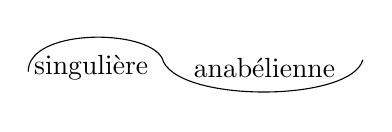
\begin{tikzpicture}[baseline=(a.base)]
\node[inner sep=1pt] (a) at (0,0) {singulière};
\node[inner sep=1pt] (b) at (2.2,0) {anabélienne};
\draw (-.8,-.05)..controls(-.8,.5)and(.7,.5)..(.9,.12)..controls(1.05,-.45)and(3.3,-.45)..(3.45,.1);
\end{tikzpicture}} donnée (sur corps $K$ de t.f. sur $\mathbb Q$), est-il vrai qu'on récupère les \unsure{él.|cl.} de \deleted{\unsure{pts}} $\operatorname{Sing}(Y)\cup\underbrace{\text{Pts marqués}}_{Y_\infty}$ en termes des \inserted{classes de conj.} sous-groupes de $\unsure{\Pi|\pi}_1(Y)$ isom. à $\widehat{\mathbb Z}$, et ext. invariants par $\unsure{\Pi|\pi}_1(K)$ (l'opération de $\unsure{\Pi|\pi}_1(K)$ dessus se fait automatiquement via le caractère cyclotomique)

c) S'inspirant des compactifications MD des $M_{g\nu}$, définir ce que c'est qu'une compactification anabélienne d'une variété lisse anabélienne (sur un corps $\inserted{K}$ de car. 0, qu'on peut supposer être de type fini sur $\mathbb Q$). Comportement par spécialisation ???
